\section{Lib\-TIM::Non\-Flat\-SE$<$ T $>$ Class Template Reference}
\label{classLibTIM_1_1NonFlatSE}\index{LibTIM::NonFlatSE@{LibTIM::NonFlatSE}}
Non-flat structuring elements (or ponderated masks).  


{\tt \#include $<$Non\-Flat\-SE.h$>$}

Inheritance diagram for Lib\-TIM::Non\-Flat\-SE$<$ T $>$::\begin{figure}[H]
\begin{center}
\leavevmode
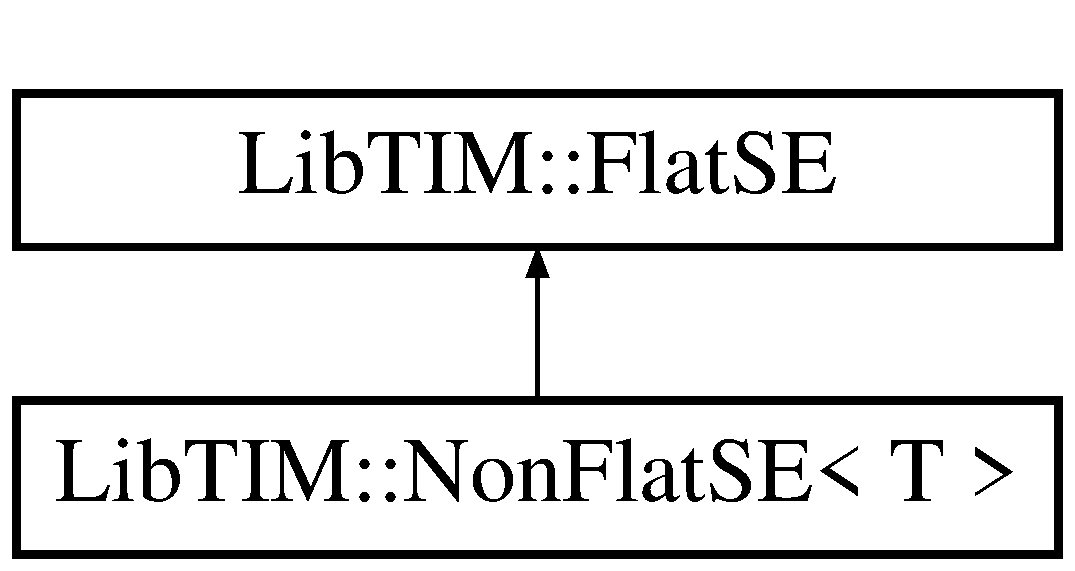
\includegraphics[height=2cm]{classLibTIM_1_1NonFlatSE}
\end{center}
\end{figure}
\subsection*{Public Member Functions}
\begin{CompactItemize}
\item 
{\bf Non\-Flat\-SE} ()
\item 
{\bf $\sim$Non\-Flat\-SE} ()
\item 
void {\bf make\-Chamfer2D} ()
\item 
{\bf Non\-Flat\-SE} {\bf raster\-Scan} ()
\item 
{\bf Non\-Flat\-SE} {\bf anti\-Raster\-Scan} ()
\item 
double {\bf get\-Norm} () const 
\item 
T {\bf get\-Value} (int i) const 
\item 
void {\bf add\-Point} ({\bf Point}$<$ {\bf TCoord} $>$ p, T attribute)
\item 
void {\bf print} ()
\item 
void {\bf reserve} (size\_\-t size)
\item 
void {\bf clear} ()
\item 
template$<$$>$ void {\bf make\-Chamfer2D} ()
\end{CompactItemize}


\subsection{Detailed Description}
\subsubsection*{template$<$class T$>$ class Lib\-TIM::Non\-Flat\-SE$<$ T $>$}

Non-flat structuring elements (or ponderated masks). 

Can be used for convolution, chanfrein masks, or non-flat morphology



\subsection{Constructor \& Destructor Documentation}
\index{LibTIM::NonFlatSE@{Lib\-TIM::Non\-Flat\-SE}!NonFlatSE@{NonFlatSE}}
\index{NonFlatSE@{NonFlatSE}!LibTIM::NonFlatSE@{Lib\-TIM::Non\-Flat\-SE}}
\subsubsection{\setlength{\rightskip}{0pt plus 5cm}template$<$class T$>$ {\bf Lib\-TIM::Non\-Flat\-SE}$<$ T $>$::{\bf Non\-Flat\-SE} ()\hspace{0.3cm}{\tt  [inline]}}\label{classLibTIM_1_1NonFlatSE_a0}


\index{LibTIM::NonFlatSE@{Lib\-TIM::Non\-Flat\-SE}!~NonFlatSE@{$\sim$NonFlatSE}}
\index{~NonFlatSE@{$\sim$NonFlatSE}!LibTIM::NonFlatSE@{Lib\-TIM::Non\-Flat\-SE}}
\subsubsection{\setlength{\rightskip}{0pt plus 5cm}template$<$class T$>$ {\bf Lib\-TIM::Non\-Flat\-SE}$<$ T $>$::$\sim${\bf Non\-Flat\-SE} ()\hspace{0.3cm}{\tt  [inline]}}\label{classLibTIM_1_1NonFlatSE_a1}




\subsection{Member Function Documentation}
\index{LibTIM::NonFlatSE@{Lib\-TIM::Non\-Flat\-SE}!addPoint@{addPoint}}
\index{addPoint@{addPoint}!LibTIM::NonFlatSE@{Lib\-TIM::Non\-Flat\-SE}}
\subsubsection{\setlength{\rightskip}{0pt plus 5cm}template$<$class T$>$ void {\bf Lib\-TIM::Non\-Flat\-SE}$<$ T $>$::add\-Point ({\bf Point}$<$ {\bf TCoord} $>$ {\em p}, T {\em attribute})\hspace{0.3cm}{\tt  [inline]}}\label{classLibTIM_1_1NonFlatSE_a7}


\index{LibTIM::NonFlatSE@{Lib\-TIM::Non\-Flat\-SE}!antiRasterScan@{antiRasterScan}}
\index{antiRasterScan@{antiRasterScan}!LibTIM::NonFlatSE@{Lib\-TIM::Non\-Flat\-SE}}
\subsubsection{\setlength{\rightskip}{0pt plus 5cm}template$<$class T$>$ {\bf Non\-Flat\-SE}$<$ T $>$ {\bf Lib\-TIM::Non\-Flat\-SE}$<$ T $>$::anti\-Raster\-Scan ()}\label{classLibTIM_1_1NonFlatSE_a4}


\index{LibTIM::NonFlatSE@{Lib\-TIM::Non\-Flat\-SE}!clear@{clear}}
\index{clear@{clear}!LibTIM::NonFlatSE@{Lib\-TIM::Non\-Flat\-SE}}
\subsubsection{\setlength{\rightskip}{0pt plus 5cm}template$<$class T$>$ void {\bf Lib\-TIM::Non\-Flat\-SE}$<$ T $>$::clear ()\hspace{0.3cm}{\tt  [inline]}}\label{classLibTIM_1_1NonFlatSE_a10}




Reimplemented from {\bf Lib\-TIM::Flat\-SE} {\rm (p.\,\pageref{classLibTIM_1_1FlatSE_a30})}.\index{LibTIM::NonFlatSE@{Lib\-TIM::Non\-Flat\-SE}!getNorm@{getNorm}}
\index{getNorm@{getNorm}!LibTIM::NonFlatSE@{Lib\-TIM::Non\-Flat\-SE}}
\subsubsection{\setlength{\rightskip}{0pt plus 5cm}template$<$class T$>$ double {\bf Lib\-TIM::Non\-Flat\-SE}$<$ T $>$::get\-Norm () const}\label{classLibTIM_1_1NonFlatSE_a5}


\index{LibTIM::NonFlatSE@{Lib\-TIM::Non\-Flat\-SE}!getValue@{getValue}}
\index{getValue@{getValue}!LibTIM::NonFlatSE@{Lib\-TIM::Non\-Flat\-SE}}
\subsubsection{\setlength{\rightskip}{0pt plus 5cm}template$<$class T$>$ T {\bf Lib\-TIM::Non\-Flat\-SE}$<$ T $>$::get\-Value (int {\em i}) const\hspace{0.3cm}{\tt  [inline]}}\label{classLibTIM_1_1NonFlatSE_a6}


\index{LibTIM::NonFlatSE@{Lib\-TIM::Non\-Flat\-SE}!makeChamfer2D@{makeChamfer2D}}
\index{makeChamfer2D@{makeChamfer2D}!LibTIM::NonFlatSE@{Lib\-TIM::Non\-Flat\-SE}}
\subsubsection{\setlength{\rightskip}{0pt plus 5cm}template$<$$>$ void {\bf Lib\-TIM::Non\-Flat\-SE}$<$ {\bf U8} $>$::make\-Chamfer2D ()\hspace{0.3cm}{\tt  [inline]}}\label{classLibTIM_1_1NonFlatSE_a11}


\index{LibTIM::NonFlatSE@{Lib\-TIM::Non\-Flat\-SE}!makeChamfer2D@{makeChamfer2D}}
\index{makeChamfer2D@{makeChamfer2D}!LibTIM::NonFlatSE@{Lib\-TIM::Non\-Flat\-SE}}
\subsubsection{\setlength{\rightskip}{0pt plus 5cm}template$<$class T$>$ void {\bf Lib\-TIM::Non\-Flat\-SE}$<$ T $>$::make\-Chamfer2D ()}\label{classLibTIM_1_1NonFlatSE_a2}


\index{LibTIM::NonFlatSE@{Lib\-TIM::Non\-Flat\-SE}!print@{print}}
\index{print@{print}!LibTIM::NonFlatSE@{Lib\-TIM::Non\-Flat\-SE}}
\subsubsection{\setlength{\rightskip}{0pt plus 5cm}template$<$class T$>$ void {\bf Lib\-TIM::Non\-Flat\-SE}$<$ T $>$::print ()\hspace{0.3cm}{\tt  [inline]}}\label{classLibTIM_1_1NonFlatSE_a8}




Reimplemented from {\bf Lib\-TIM::Flat\-SE} {\rm (p.\,\pageref{classLibTIM_1_1FlatSE_a28})}.\index{LibTIM::NonFlatSE@{Lib\-TIM::Non\-Flat\-SE}!rasterScan@{rasterScan}}
\index{rasterScan@{rasterScan}!LibTIM::NonFlatSE@{Lib\-TIM::Non\-Flat\-SE}}
\subsubsection{\setlength{\rightskip}{0pt plus 5cm}template$<$class T$>$ {\bf Non\-Flat\-SE}$<$ T $>$ {\bf Lib\-TIM::Non\-Flat\-SE}$<$ T $>$::raster\-Scan ()}\label{classLibTIM_1_1NonFlatSE_a3}


\index{LibTIM::NonFlatSE@{Lib\-TIM::Non\-Flat\-SE}!reserve@{reserve}}
\index{reserve@{reserve}!LibTIM::NonFlatSE@{Lib\-TIM::Non\-Flat\-SE}}
\subsubsection{\setlength{\rightskip}{0pt plus 5cm}template$<$class T$>$ void {\bf Lib\-TIM::Non\-Flat\-SE}$<$ T $>$::reserve (size\_\-t {\em size})\hspace{0.3cm}{\tt  [inline]}}\label{classLibTIM_1_1NonFlatSE_a9}




Reimplemented from {\bf Lib\-TIM::Flat\-SE} {\rm (p.\,\pageref{classLibTIM_1_1FlatSE_a29})}.

The documentation for this class was generated from the following files:\begin{CompactItemize}
\item 
Common/{\bf Non\-Flat\-SE.h}\item 
Common/{\bf Non\-Flat\-SE.hxx}\end{CompactItemize}
